\documentclass[]{article}
\usepackage{lmodern}
\usepackage{amssymb,amsmath}
\usepackage{ifxetex,ifluatex}
\usepackage{fixltx2e} % provides \textsubscript
\ifnum 0\ifxetex 1\fi\ifluatex 1\fi=0 % if pdftex
  \usepackage[T1]{fontenc}
  \usepackage[utf8]{inputenc}
\else % if luatex or xelatex
  \ifxetex
    \usepackage{mathspec}
  \else
    \usepackage{fontspec}
  \fi
  \defaultfontfeatures{Ligatures=TeX,Scale=MatchLowercase}
\fi
% use upquote if available, for straight quotes in verbatim environments
\IfFileExists{upquote.sty}{\usepackage{upquote}}{}
% use microtype if available
\IfFileExists{microtype.sty}{%
\usepackage{microtype}
\UseMicrotypeSet[protrusion]{basicmath} % disable protrusion for tt fonts
}{}
\usepackage[margin=2cm]{geometry}
\usepackage{hyperref}
\hypersetup{unicode=true,
            pdftitle={The title},
            pdfauthor={Richard Pilbery},
            pdfborder={0 0 0},
            breaklinks=true}
\urlstyle{same}  % don't use monospace font for urls
\usepackage{natbib}
\bibliographystyle{apalike}
\usepackage{longtable,booktabs}
\usepackage{graphicx,grffile}
\makeatletter
\def\maxwidth{\ifdim\Gin@nat@width>\linewidth\linewidth\else\Gin@nat@width\fi}
\def\maxheight{\ifdim\Gin@nat@height>\textheight\textheight\else\Gin@nat@height\fi}
\makeatother
% Scale images if necessary, so that they will not overflow the page
% margins by default, and it is still possible to overwrite the defaults
% using explicit options in \includegraphics[width, height, ...]{}
\setkeys{Gin}{width=\maxwidth,height=\maxheight,keepaspectratio}
\IfFileExists{parskip.sty}{%
\usepackage{parskip}
}{% else
\setlength{\parindent}{0pt}
\setlength{\parskip}{6pt plus 2pt minus 1pt}
}
\setlength{\emergencystretch}{3em}  % prevent overfull lines
\providecommand{\tightlist}{%
  \setlength{\itemsep}{0pt}\setlength{\parskip}{0pt}}
\setcounter{secnumdepth}{5}
% Redefines (sub)paragraphs to behave more like sections
\ifx\paragraph\undefined\else
\let\oldparagraph\paragraph
\renewcommand{\paragraph}[1]{\oldparagraph{#1}\mbox{}}
\fi
\ifx\subparagraph\undefined\else
\let\oldsubparagraph\subparagraph
\renewcommand{\subparagraph}[1]{\oldsubparagraph{#1}\mbox{}}
\fi

%%% Use protect on footnotes to avoid problems with footnotes in titles
\let\rmarkdownfootnote\footnote%
\def\footnote{\protect\rmarkdownfootnote}

%%% Change title format to be more compact
\usepackage{titling}

% Create subtitle command for use in maketitle
\newcommand{\subtitle}[1]{
  \posttitle{
    \begin{center}\large#1\end{center}
    }
}

\setlength{\droptitle}{-2em}
  \title{The title}
  \pretitle{\vspace{\droptitle}\centering\huge}
  \posttitle{\par}
  \author{Richard Pilbery}
  \preauthor{\centering\large\emph}
  \postauthor{\par}
  \predate{\centering\large\emph}
  \postdate{\par}
  \date{2019-01-25}

\usepackage{booktabs}
\usepackage{amsthm}
\makeatletter
\def\thm@space@setup{%
  \thm@preskip=8pt plus 2pt minus 4pt
  \thm@postskip=\thm@preskip
}
\makeatother
\usepackage{booktabs}
\usepackage{longtable}
\usepackage{array}
\usepackage{multirow}
\usepackage[table]{xcolor}
\usepackage{wrapfig}
\usepackage{float}
\usepackage{colortbl}
\usepackage{pdflscape}
\usepackage{tabu}
\usepackage{threeparttable}
\usepackage[normalem]{ulem}

\AtBeginDocument{\let\maketitle\relax}

\begin{document}
\maketitle

{
\setcounter{tocdepth}{2}
\tableofcontents
}
\hypertarget{the-title-goes-here}{%
\section{The title goes here}\label{the-title-goes-here}}

\hypertarget{author-information}{%
\subsection{Author information}\label{author-information}}

\textbf{Richard Pilbery}\\
Research paramedic\\
Yorkshire Ambulance Service NHS Trust\\
Springhill, Brindley Way\\
Wakefield 41 Business Park\\
Wakefield\\
WF2 0XQ

ORCID: \url{https://orcid.org/0000-0002-5797-9788}

email: \href{mailto:r.pilbery@nhs.net}{\nolinkurl{r.pilbery@nhs.net}}\\
tel:

\textbf{Word count:} 1074

\textbf{Keywords:} Keyword 1, keyword 2, keyword 3

\hypertarget{abstract}{%
\subsection{Abstract}\label{abstract}}

\hypertarget{introduction}{%
\subsubsection{Introduction}\label{introduction}}

Intro

\hypertarget{methods}{%
\subsubsection{Methods}\label{methods}}

Methods

\hypertarget{results}{%
\subsubsection{Results}\label{results}}

Results

\hypertarget{conclusion}{%
\subsubsection{Conclusion}\label{conclusion}}

Conclusion

\hypertarget{intro}{%
\section{Introduction}\label{intro}}

Vomiting and regurgitation are commonly encountered in
out-hospital-cardiac arrest with a reported incidence of 20--30\%
\citep{voss_how_2014, simons_incidence_2007}. This is of concern since
patients who have suffered an OHCA, are already in extremis. If standard
suctioning techniques are not sufficient to maintain a clear airway and
provide ventilation, then these patients will die, irrespective of the
quality of chest compressions and the timeliness of defibrillation.
Arguably, tracheal intubation is the preferred airway management
technique in patients with ongoing airway contamination, but there is
evidence that this is difficult to achieve when the airway is soiled
\citep{sakles_impact_2017}. Even if patients survive to the hospital, it
is possible that aspiration pneumonias may adversely affect survival
outcome, although this has yet to be proved empirically
\citep{christ_early-onset_2016}.

Traditional suctioning techniques have been criticised, and training in
the management of contaminated airways, limited. This has led to the
development of a combined suction/laryngoscopy technique to facilitate
intubation, known as Suction Assisted Laryngoscopy and Airway
Decontamination (SALAD), and the creation of modified airway manikins to
allow for practice in these techniques \citep{ducanto_novel_2017}.

However, to date there has only been one study specifically looking at
the SALAD technique and the outcomes were self-reported confidence
measures of trainees in using the technique. Other techniques have been
described to manage significant airway contamination, including the use
of a meconium aspirator \citep{kei_comparing_2017}, which is not
practical in the out-of-hospital environment (and requires a device that
is not typically carried by UK ambulance services), and deliberate
intubation of the oesophagus (the oesophageal diversion manoeuvre), of
which the sum total of evidence in support of the procedure is a single
case report \citep{kornhall_intentional_2015}.

This study aims to determine whether a short teaching session of the
SALAD technique to paramedics, improves their ability to intubate a
contaminated airway.The primary objective is to determine the difference
between paramedic first-pass intubation success, before and after SALAD
training, in a simulated soiled airway. Secondary objectives are to
determine the difference in time taken to achieve first-pass intubation
success, before and after SALAD training in a simulated soiled airway,
and the effect of multiple intubation attempts on success rates
following SALAD training.

\hypertarget{methods-1}{%
\section{Methods}\label{methods-1}}

\hypertarget{study-design-and-participants}{%
\subsection{Study design and
participants}\label{study-design-and-participants}}

This randomised controlled trial was conducted in Yorkshire Ambulance
Service NHS Trust (YAS). Participants were NHS staff employed by YAS,
who were Health and Care Professions Council (HCPC) registered
paramedics at the time of enrolment in the study, authorised to intubate
and who had received no SALAD training in the previous 3 months.
Potential participants were excluded if they did not meet the inclusion
criteria, were allergic to the `vomit' ingredients or unwilling to
provide consent to participate.

\hypertarget{randomisation}{%
\subsection{Randomisation}\label{randomisation}}

In order to adjust for changes in participant performance by making
repeated attempts at intubation, paramedics were randomised into either:
making two pre-training intubation attempts and one post-training
attempt (group AAB); or making one pre-training intubation attempt and
two post-training attempts (ABB). Groups were evenly allocated
(i.e.~1:1) using a block randomisation sequence provided by RANDOM.ORG.
To distinguish between the training pathways and number of the assessed
attempts, group AAB's attempts were denoted
A\textsubscript{01}A\textsubscript{02}B\textsubscript{01} and group
ABBs, A\textsubscript{11}B\textsubscript{11}B\textsubscript{12}.

\hypertarget{intervention}{%
\subsection{Intervention}\label{intervention}}

\hypertarget{salad-manikin}{%
\subsubsection{SALAD manikin}\label{salad-manikin}}

A modified TruCorp AirSim Advance airway manikin was used for the study
as it has realistic airway anatomy and can be used for tracheal
intubation training. The oesophagus of this manikin has been connected,
via a hosepipe, to a bilge pump that is sited within a reservoir of
simulated vomit (Figure \ref{fig:figure1}). The vomit is water, coloured
with food-grade colouring, and thickened with xanthan gum (a food
additive). Once the bilge pump is switched on, it can generate a
constant flow of liquid into the oropharynx, obscuring any view of the
laryngeal inlet. The flow rate is controlled by a tap, which was
calibrated to provide 1 L/min of vomit to the oropharynx of the manikin
during intubation attempts. To keep vomit within the oropharynx, the
left and right bronchi on the manikin have been occluded.

Standard intubation equipment, including personal protective equipment
(PPE) and motorised suction, that is routinely used within YAS was
provided for participants, and the study researcher acted as a competent
assistant for the intubation attempts.

\begin{figure}
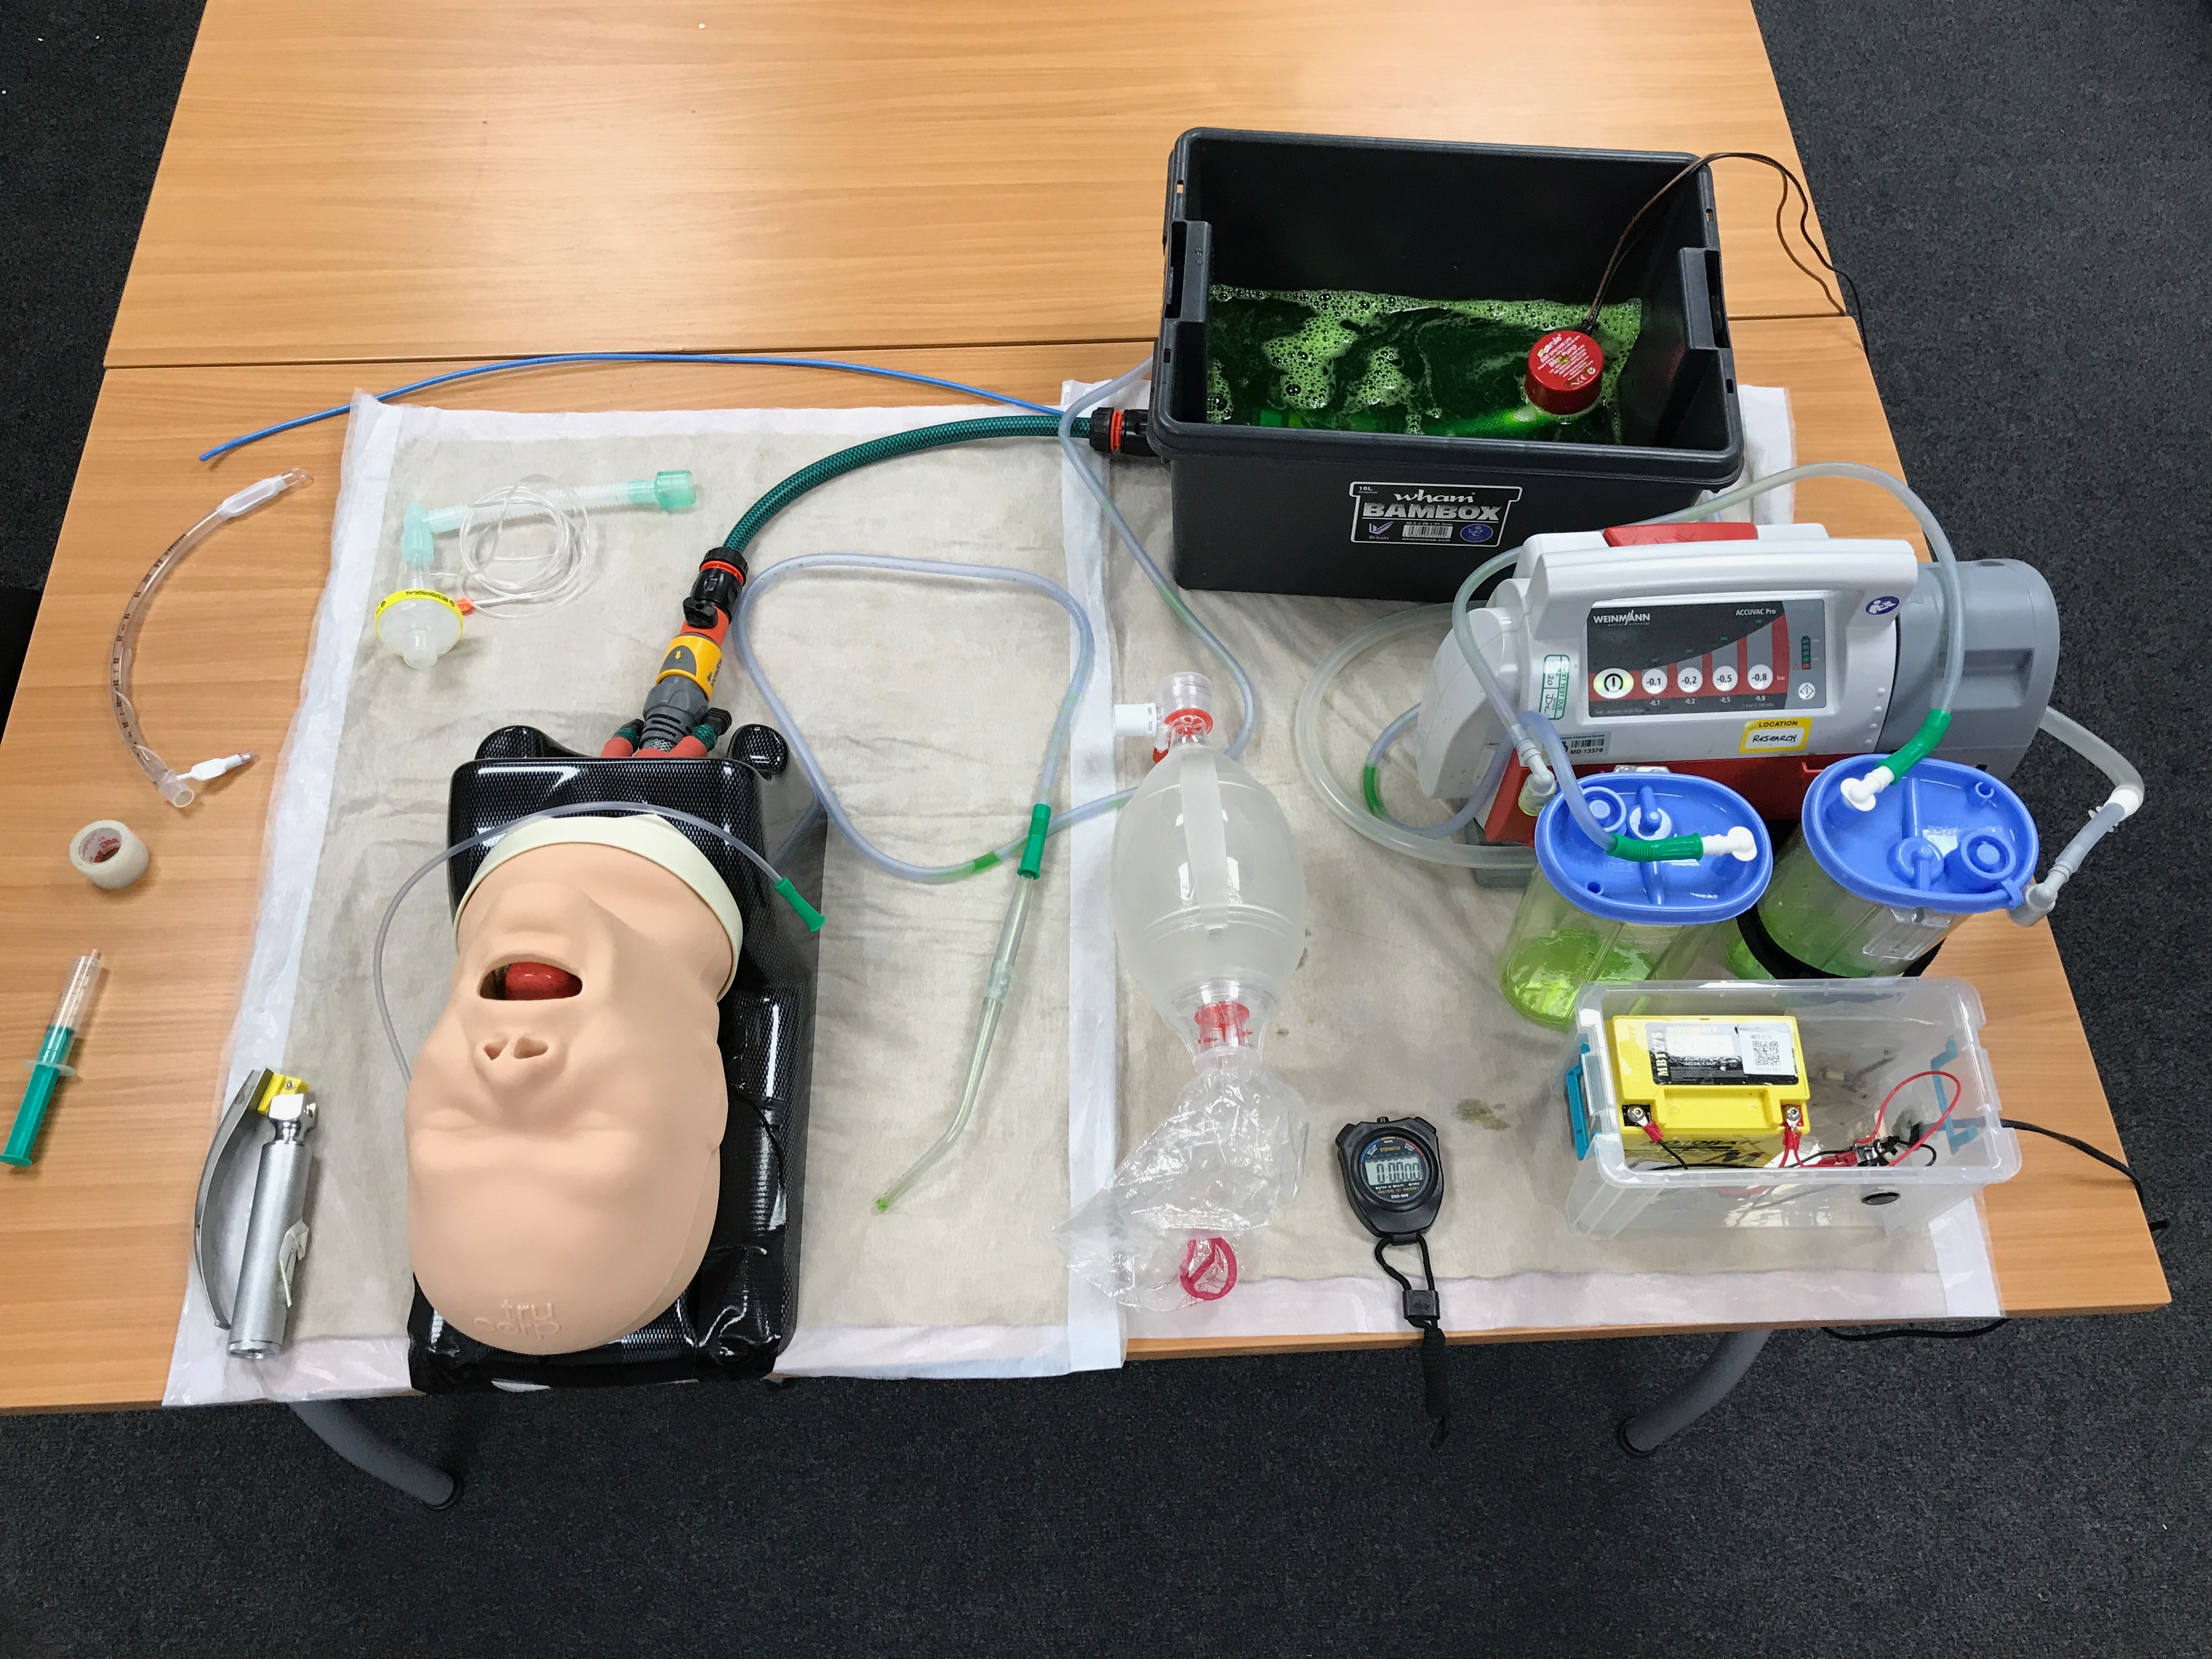
\includegraphics[width=7in]{images/figure-1} \caption{SALAD manikin setup used for the study}\label{fig:figure1}
\end{figure}

\hypertarget{procedure}{%
\subsubsection{Procedure}\label{procedure}}

Once informed consent was obtained, paramedics were randomised into
either: group AAB where they made two pre-training and one post-training
attempts, or ABB, where one pre-training and two post-training attempts
were undertaken. All attempts utilised direct laryngoscopy, which is the
standard intubation technique within YAS. Prior to each intubation
attempt, the manikin was primed with vomit to ensure the same level of
oropharyngeal obstruction. All attempts were video recorded for timing
accuracy.

Participants were deemed to have begun their attempt once the bilge pump
was turned on. The attempt will be considered over when either: the
paramedic intubates the manikin and verbally confirms with the
researcher that the attempt has been completed or; 90 seconds has
elapsed or; the tracheal tube is placed into the oesophagus and the cuff
is inflated while the pump is still running.

If the tracheal tube was not in the trachea, with the cuff inflated and
connected to a bag-valve device within 90 seconds, the attempt was
considered a failure.

Participants randomised into the two pre-training attempts group (AAB)
made their second intubation attempt immediately following the first,
and prior to the group training session. Once all participants completed
their pre-training intubation attempt(s), the training session was
delivered. The training intervention adopted the Advanced Life Support
Group/Resuscitation Council 4-stage approach of skills teaching,
comprising \citep{bullock_pocket_2008}:

\begin{enumerate}
\def\labelenumi{\arabic{enumi}.}
\tightlist
\item
  A real-time demonstration of the SALAD technique by the researcher
\item
  A repeated demonstration with an explanation of the rationale of the
  steps taken when performing SALAD (not real-time)
\item
  Another demonstration of the SALAD technique conducted by the
  researcher, but guided by one of the participants
\item
  An attempt by the same participant who guided the researcher in the
  previous step, followed by a practice attempt by the other
  participants.
\end{enumerate}

Following the training session, participants made their post-training
intubation attempt(s) conducted using the same method as for the
pre-training intubation attempt(s). Participants randomised into the two
post-training attempts (ABB), made their second attempt immediately
following the first post-training attempt.

\hypertarget{outcomes}{%
\subsection{Outcomes}\label{outcomes}}

\hypertarget{sample-size}{%
\subsection{Sample size}\label{sample-size}}

\hypertarget{randomisation-1}{%
\subsection{Randomisation}\label{randomisation-1}}

\hypertarget{results-1}{%
\section{Results}\label{results-1}}

\hypertarget{discussion}{%
\section{Discussion}\label{discussion}}

Discussion blurb

\hypertarget{conclusion-1}{%
\section{Conclusion}\label{conclusion-1}}

The conclusion

\hypertarget{appendix-a}{%
\section{Appendix A}\label{appendix-a}}

Appendix (if you need one)

\bibliography{references.bib,packages.bib}


\end{document}
